% Une première expérimentation pour EHRI : l'application DiScholEd

\section{Une application pour publier les ego-documents}

\subsection{Qu'est-ce qu'un ego-document ?}
La mention d'\enquote{ego-document} apparaît dans les années 1950, utilisée par l'historien néerlandais Jacques Presser pour décrire les textes sur lesquels se basent ses recherches~: des journaux intimes, mémoires, autobiographies et de la correspondance personnelle (\enquote{\textit{Ego-Dokument}  \footcite[p.~46]{AltedVigil2022}}). Le terme \enquote{ego-document} est plus largement employé dans le monde anglophone~; en France, on entendra volontiers parler d'\enquote{écrits du for privé\footnote{Juliette Deloye, \enquote{For privé (écrits du)} dans VOCES, \textit{Vocabulaire pour l'Étude des Scripturalités}, Thomas Brunner (dir.), ARCHE UR3400 (Université de Strasbourg), édition électronique, 2019, \texttt{DOI~: \href{https://doi.org/10.34931/vvxh-5046}{10.34931/vvxh-5046}} (visité le 03/09/2023).}} ou d'\enquote{écriture de soi}. L'étude des ego-documents s'inscrit dans le courant historiographique de l'\enquote{Histoire par le bas} (\enquote{\textit{History From Below}}).


\subsection{Les collections publiées sur DiScholEd}
À ce jour, l'application DiScholEd\footcite{DiScholEd} compte sept collections. Nous présenterons ici les plus documentées par l'application. L'une d'entre elles, la collection \enquote{\textit{Early Holocaust Testimony} de l'EHRI}, nous intéressera particulièrement.  

\subsubsection*{Correspondance de Paul d'Estournelles de Constant}
Paul d’Estournelles de Constant (1852-1924) était un homme politique français. Il devient sénateur en 1905, fonction qu'il occupera jusqu'à sa mort. Prix Nobel de la paix, il a \oe{}uvré pour le maintien de la paix entre les pays, notamment avec la Grande-Bretagne et l'Allemagne. Le corpus est composé de sa correspondance pendant la Première Guerre mondiale. Paul d'Estournelles de Constant y apporte son point de vue en tant qu'élu, mais aussi en tant que citoyen et père de famille\footcite[collection \enquote{Correspondance de Paul d'Estournelles de Constant}, section \enquote{\textit{History of the Corpus}} (visité le 03/09/2023)]{DiScholEd}.  

\subsubsection*{Intellectuels Berlinois}
Le collection \enquote{Lettres et textes: Le Berlin intellectuel des années 1800} témoigne de la vie intellectuelle berlinoise de la fin du XVIII\ieme{} et du début du XIX\ieme{} siècle. Le corpus met en avant le développement du romantisme allemand et les relations que les cercles intellectuels berlinois entretenaient entre eux\footcite[collection \enquote{Lettres et textes: Le Berlin intellectuel des années 1800}, section \enquote{\textit{History of the Corpus}} (visité le 03/09/2023)]{DiScholEd}.

\subsubsection*{Catalogue des manuscrits d'Auguste Boeckh}
Auguste Boeckh (1785-1867) était un philologue allemand. Il a enseigné à l'université de Berlin, avant de devenir le doyen de la faculté des Arts et Sciences Humaines. La collection est composée du catalogue de ses manuscrits, réunis dans le cadre du projet \enquote{\textit{Boeckh-Nachlassprojekt\footcite[collection \enquote{Catalogue des manuscrits d'Auguste Boeckh}, section \enquote{\textit{History of the Corpus}} (visité le 03/09/2023)]{DiScholEd}}}.  



\section{La collection \enquote{\textit{Early Holocaust Testimony}} sur DiScholEd}
Le contenu de la collection \enquote{\textit{Early Holocaust Testimony}} sur DiScholEd est identique à celui de l'édition publiée avec Omeka\footnote{Consultable à l'adresse~: \texttt{\href{https://early-testimony.ehri-project.eu/}{https://early-testimony.ehri-project.eu/}}.}, seul l'affichage est différent. La simplicité de l'affichage proposé par TEI Publisher nous permet de présenter l'édition en donnant accès à l'utilisateur$\cdot$ice aux informations sur l'édition et sur l'EHRI, aux textes édités et aux index directement depuis la page d'accueil (Figure \ref{fig:ehri-discholed-accueil}). La présentation de la collection (section \enquote{Texts édités}) permet de naviguer directement dans toute la collection (Figure \ref{fig:ehri-discholed-collection}), alors que le site Omeka ne propose que d'explorer les exemples proposés par les éditeur$\cdot$ice$\cdot$s dans un premier temps.  

La disposition horizontale (Figure \ref{fig:doc-teipublisher}) permet d'afficher plusieurs vues d'une importance équivalente, alors que la présentation de la transcription sur Omeka se fait au détriment du fac-similé (Figure \ref{fig:ehri-omeka}), dont l'affichage nous semble tout particulièrement pertinent au sein d'une édition numérique de documents d'archives.

\begin{figure}[h]
    \centering
    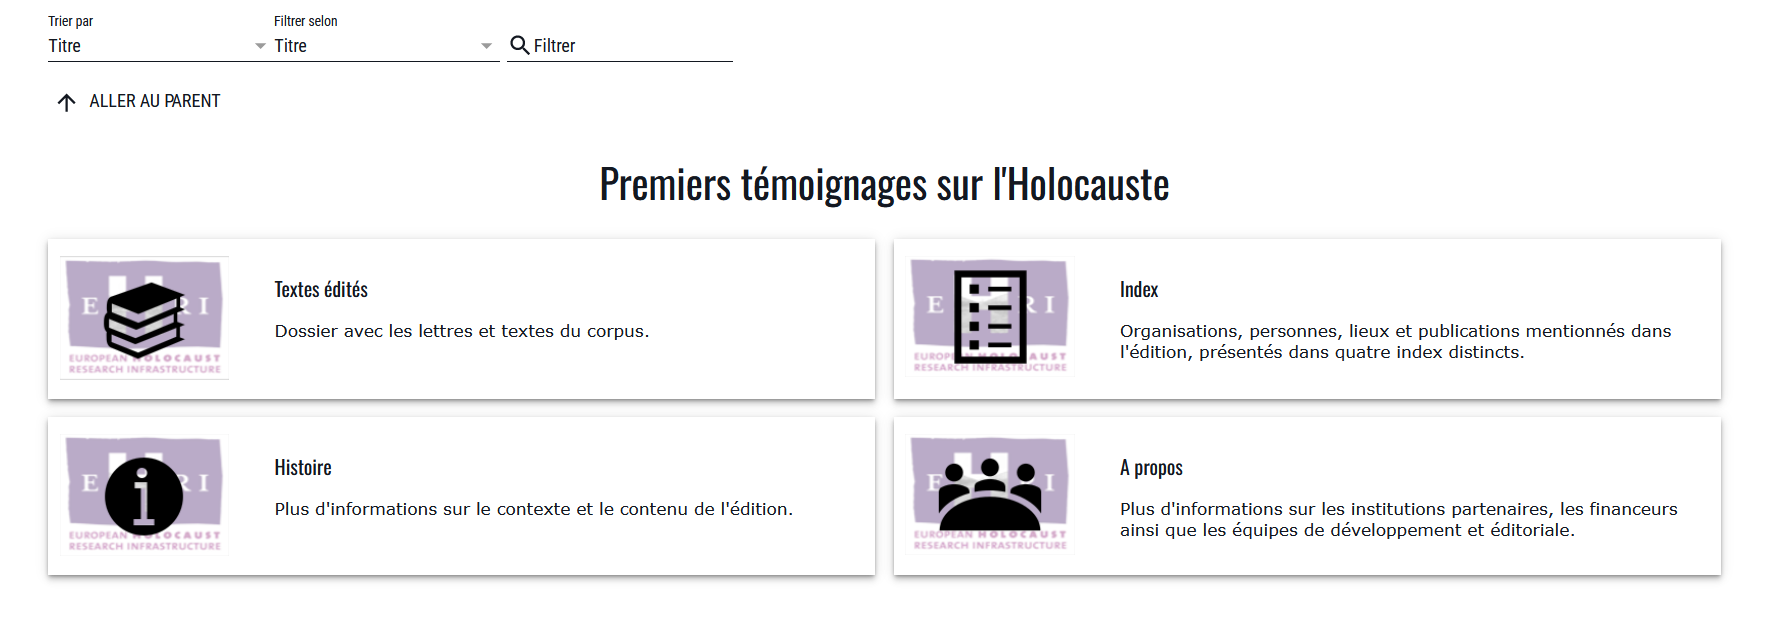
\includegraphics[width=1\linewidth]{2-MAIN/images/discholed-accueil.png}
    \caption{Page d'accueil de la collection sur DiScholEd}
    \label{fig:ehri-discholed-accueil}
\end{figure}

\begin{figure}[h]
    \centering
    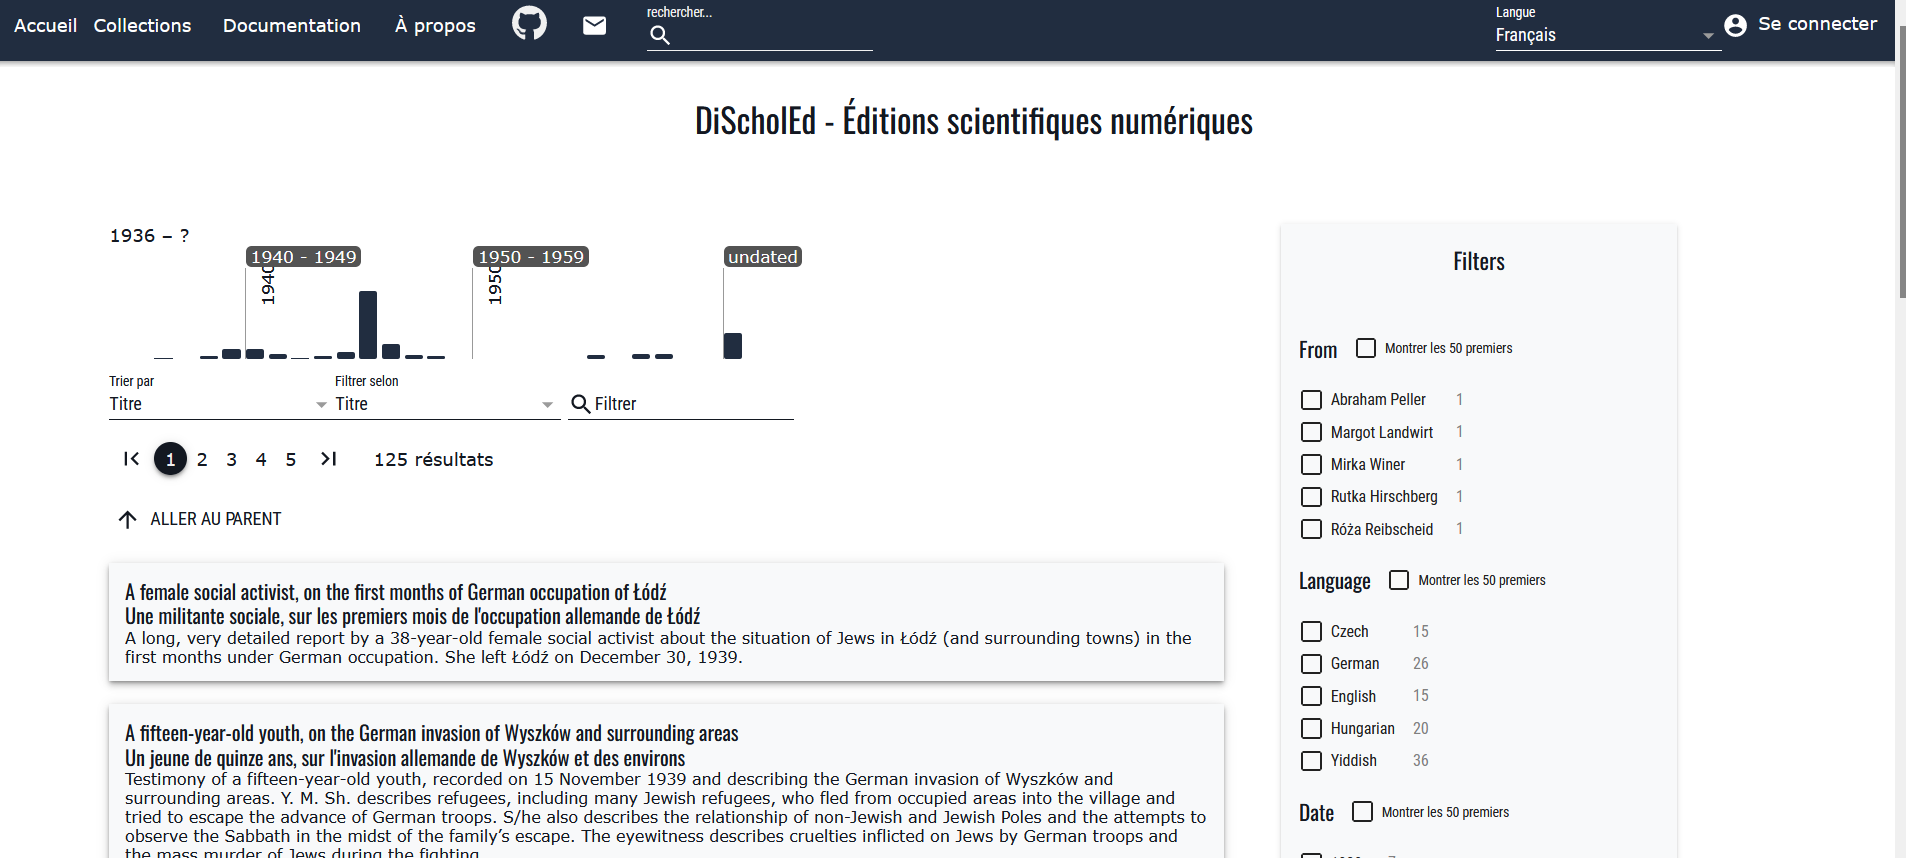
\includegraphics[width=1\linewidth]{2-MAIN/images/discholed-collection.png}
    \caption{Collection \enquote{\textit{Early Holocaust Testimony}} sur DiScholEd}
    \label{fig:ehri-discholed-collection}
\end{figure}

\bigskip
\bigskip
La publication de la collection \enquote{\textit{Early Holocaust Testimony}} sur DiScholEd a permis à l'équipe éditoriale du WP12 d'avoir une idée du rendu des éditions qu'elle pourrait y publier. La compatibilité naturelle de TEI Publisher avec les fichiers encodés en TEI permet à la communauté de développer des modules plus simples à incorporer à son projet. En outre, TEI Publisher dispose d'un outil d'annotation intégré dont la maîtrise optimiserait davantage le travail éditorial.